\chapter{Vybrané zbernicové protokoly}
\label{kap:protokoly}

V tejto kapitole stručne spomenieme vybrané zbernicové protokoly a zhrnieme ich kľúčové vlastnosti, ktoré budú relevantné v ďalších častiach práce. Vo všeobecnosti existuje mnoho rôznych zbernicových protokolov. Tie môžu využívať rôzne techniky, ktoré umožňujú zabezpečiť komunikáciu a jej riadenie. Mnoho týchto protokolov má však veľa spoločných znakov. Aj preto sa v práci budeme venovať iba niektorým vybraným. V tejto kapitole uvedieme príklad zbernice, ktorej súčasťou je štandardizovaný protokol pre komunikáciu (I$^2$C), príklad defakto-štandardu SPI a konkrétny príklad implementácie SPI zbernice pre komunikáciu s vybranou EEPROM pamäťou AT93C66A. Spomenuté zbernice sú široko používané najmä v kontexte vnorených zariadení z dôvodu nízkeho výkonu zbernice a spotreby energie.

\section{I$^2$C Zbernica}
I$^2$C (Inter-Integrated Circuits) je štandardizovaná zbernica, vyvinutá spoločnosťou Philips Semiconductors, určená pre jednoduchú komunikáciu medzi integrovanými obvodmi \cite{i2cBus} väčšinou v rámci jednej dosky plošných spojov. Ide o bitovo-orientovanú synchrónnu linku, čo znamená, že komunikácia je synchronizovaná hodinovými impulzmi a prenášaná dátová jednotka je bit.

\subsection{Hardvér I$^2$C zbernice}
Zbernica pozostáva z dvoch vodičov: SDA (Serial Data Line), ktorý zabezpečuje sériový prenos dát (bitov) a SCL (Serial Clock Line) pre prenos synchronizačného hodinového signálu \cite{i2cBus}. Vodiče sú na komunikujúcich zariadeniach pripojené v tzv. open-drain režime a (každé zvlášť) sú cez zdvíhací odpor (pull-up rezistor) pripojené k napätiu 5\,V resp. 3.3\,V v závislosti od konfigurácie. Na obrázku \ref{obr:i2cWiring} je znázornené zapojenie zariadení pomocou zbernice I$^2$C.

\begin{figure}
    \centerline{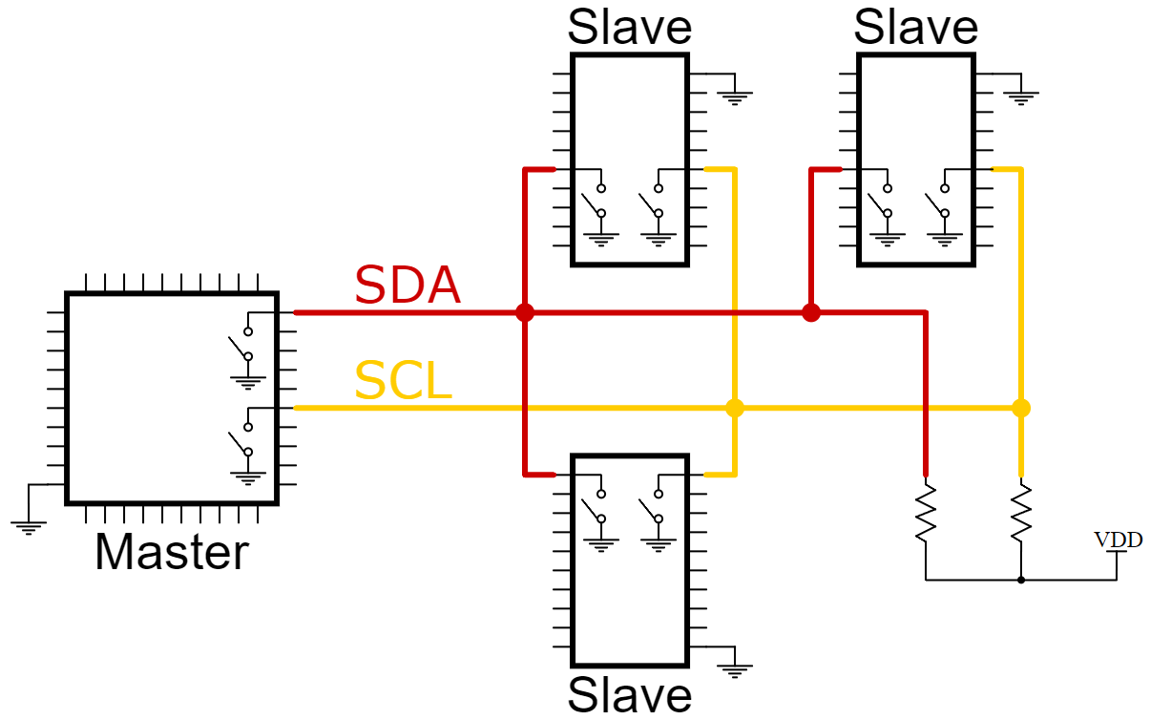
\includegraphics[width=0.9\textwidth]{images/i2cWiring.png}}
    \caption[Zapojenie zbernice I$^2$C]{Zapojenie zbernice I$^2$C. Open-drain logika interného zapojenia vodičov v zariadeniach je znázornená pomocou \uv{vypínačov}. V skutočnosti je realizovaná pomocou tranzistorov.}
    \label{obr:i2cWiring}
\end{figure}

V pasívnom stave je teda na vodičoch hodnota napätia 5\,V (resp. 3.3\,V), čo na dátovej linke zodpovedá logickej hodnote 1. V prípade, že práve vysielajúce zaradenie chce poslať bit s logickou hodnotou 0, \uv{pripojí} (napr. pomocou tranzistora) vodič na spoločnú zem, čím napätie klesne na 0\,V. Dáta na vodiči SDA sú vzorkované pri nábehovej hrane na SCL signálovej linke \cite{i2cBus}.

\subsection{Riadenie prístupu k zbernici}
Zbernica I$^2$C je typu half-duplex, podporuje teda obojsmernú komunikáciu, pričom súčasne môže komunikácia prebiehať iba jedným smerom. Komunikácia na I$^2$C zbernici je riadená architektúrou master-slave \cite{i2cBus}. Master zariadenie riadi komunikáciu na hardvérovej aj protokolovej úrovni. Na hardvérovej úrovni master zariadenie určuje rýchlosť komunikácie generovaním hodinových impulzov na SDL vodiči. Zbernica podporuje rôzne konfigurácie, ktoré sa líšia rýchlosťou rádovo od 100\,kbps až po niekoľko\,Mbps. Na protokolovej úrovni je každá komunikácia iniciovaná aj ukončená master zariadením a slave zariadenia musia synchrónne posielať dáta vo vyhradených časoch, ktoré definuje protokol.

\subsection{Protokol a štruktúra rámcov}
I$^2$C je zbernica so zdieľaným médiom, čo znamená, že umožňuje na spoločnú zbernicu pripojiť viacej než dva komunikujúce uzly. Je preto potrebné zabezpečiť adresáciu jednotlivých zariadení, s ktorými chce master nadviazať komunikáciu. Každé slave zariadenie má pridelenú 7-bitovú (resp. 10-bitovú v novšej verzii štandardu) adresu, ktorá je zvyčajne zadrôtovaná výrobcom hardvéru \cite{i2cBus}. Z dôvodu predchádzania kolízií v adresách, zvyknú výrobcovia prideliť zariadeniu viacero adries, z ktorých je možne nakonfigurovať práve jednu, väčšinou hardvérovým spínačom.

Samotná komunikácia vyzerá nasledovne: Master zariadenie nastaví úroveň napätia na SDA linke na hodnotu logickej 0, čím pošle tzv. START bit, ktorý signalizuje začiatok komunikácie. Nasleduje 7-bitová (resp. 10-bitová) adresa zariadenia, s ktorým chce master komunikovať a jeden tzv R/W bit, ktorý označuje, či ide o operáciu čítania alebo zápisu. (Z pohľadu master zariadenia logická 1 predstavuje čítanie, 0 predstavuje zápis.) S nasledujúcim hodinovým impulzom musí adresované slave zariadenie komunikáciu potvrdiť (pošle tzv. ACK bit) tým, že úroveň napätia na SDA linke nastaví na hodnotu logickej 0. Potom nasledujú samotné dáta, ktoré posiela master (resp. slave v prípade, že ide o operáciu čítania). Dáta su členené na 8-bitové sekvencie, ktoré sú zakaždým potvrdzované druhou stranou rovnakým spôsobom. Za posledným potvrdením dát pošle master tvz. STOP bit, čím signalizuje ukončenie komunikácie. Štruktúra rámca je znázornená na obrázku \ref{obr:i2cFrame}.

\begin{figure}
    \centerline{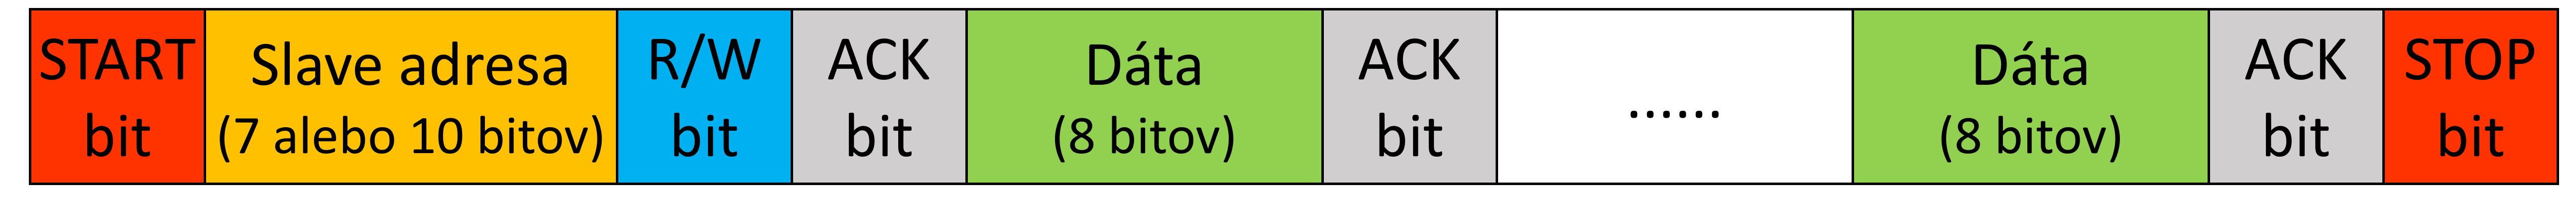
\includegraphics[width=1\textwidth]{images/i2cFrame.png}}
    \caption[Štruktúra I$^2$C rámca]{Štruktúra I$^2$C rámca.}
    \label{obr:i2cFrame}
\end{figure}

V prípade, že počas komunikácie nastane chyba, prijímajúce zariadenie nepošle ACK bit. Teda napätie na SDA linke ostane na úrovni logickej 1 (tzv. NACK bit), čo je zároveň pasívny stav. V takomto prípade môže master reagovať dvoma spôsobmi. Buď pošle STOP bit, čo znamená okamžité ukončenie komunikácie, alebo môže zopakovať komunikáciu od začiatku, tým, že pošle START bit. Postupnosť NACK a STOP môže byť master zariadením zároveň využitá na signalizáciu ukončenia komunikácie v prípade operácie čítania \cite{i2cBus}.

\subsection{Mechanizmus naťahovania hodín}
Naťahovanie hodín (angl. clock stretching) je mechanizmus I$^2$C protokolu, ktorý umožňuje slave zariadeniu dočasne spomaliť hodinové impulzy generované master zariadením \cite{i2cBus}. To umožňuje slave zariadeniu spomaliť rýchlosť komunikácie, v prípade potreby väčšieho času pre spracovanie dát.

Počas prebiehajúcej komunikácie master zariadenie monitoruje vysielaný hodinový signál na SCL linke. Pripomíname, že vodič SCL linky je pripojený cez zdvíhací odpor k zdroju napätia a komunikujúce zariadenia majú vodič pripojený v open-drain režime. Pokiaľ chce slave zariadenie spomaliť komunikáciu môže podržať SCL vodič pripojený na zem, čím dosiahne efekt, že napätie na vodiči ostane na úrovni logickej 0 aj v prípade, že master posiela logickú 1. Tento stav dokáže master detegovať a následne prispôsobiť rýchlosť hodinových impulzov, čím spomalí komunikáciu. Mechanizmus naťahovania hodín je znázornený na obrázku \ref{obr:i2cStretch}.

\begin{figure}
    \centerline{
\includegraphics[width=0.8\textwidth]{images/i2cStretch.png}}
    \caption[Mechanizmus naťahovania hodín]{Mechanizmus naťahovania hodín. Na vrchnej časti je pôvodný hodinový signál vysielaný master zariadením. Na spodnej je skutočný signál po natiahnutí hodín slave zariadením.}
    \label{obr:i2cStretch}
\end{figure}

\noindent<COMMENT>\\ 
\textit{Mohlo by byť zaujímavé skúsiť sa pozrieť, či sa toto nedá zneužiť práve na \uv{legálne} spomalenie komunikácie, v prípade, že nestíhame realizovať MITM útok.}\\
<COMMENT>

\section{SPI Zbernica}
Zbernica SPI je defakto-štandard, ktorý definuje hardvérové rozhranie, pre zapojenie komunikujucích strán. Podobne ako I$^2$C, ide o bitovo orientovanú synchrónnu linku. Keďže ide o defakto-štandard, zbernica SPI nedefinuje predpísanú štruktúru posielaných dát \cite{spiBus}.

\subsection{Riadenie prístupu k zbernici}
Podobne ako pri I$^2$C zbernici, komunikácia je riadená master-slave architektúrou. Prístup k zbernici riadi master prostredníctvom dedikovaného vodiča SS (Slave Select) pre každé slave zariadenie. Vodiče SS zvyknú byť označené aj ako CS (Chip Select). V pasívnom stave je na každom SS vodiči logická hodnota 1. Pred začatím komunikácie s vybraným slave zariadením nastaví master logickú hodnotu 0 na príslušnom SS vodiči, čím umožní komunikáciu medzi master a príslušným slave zariadením. Tento spôsob riadenia zbernice vytvára ilúziu point-to-point linky medzi komunikujúcimi stranami, preto v zbernici SPI nie je potrebná adresácia.

\subsection{Hardvér SPI zbernice}
SPI zbernica pozostáva z troch hlavných liniek: MISO (Master In Slave Out), ktorý zabezpečuje prenos dát smerom od slave zariadení k master zariadeniu, MOSI (Master Out Slave In) pre prenos dát opačným smerom a SCLK (Serial Clock) pre prenos hodinového signálu (generovaný master zariadením) \cite{spiBus}. Schéma zapojenia pomocou SPI zbernice je na obrázku \ref{obr:spiWiring}. Dáta po vodičoch MISO a MOSI môžu tiecť súčasne čo umožňuje full-duplex komunikáciu.

\begin{figure}
    \centerline{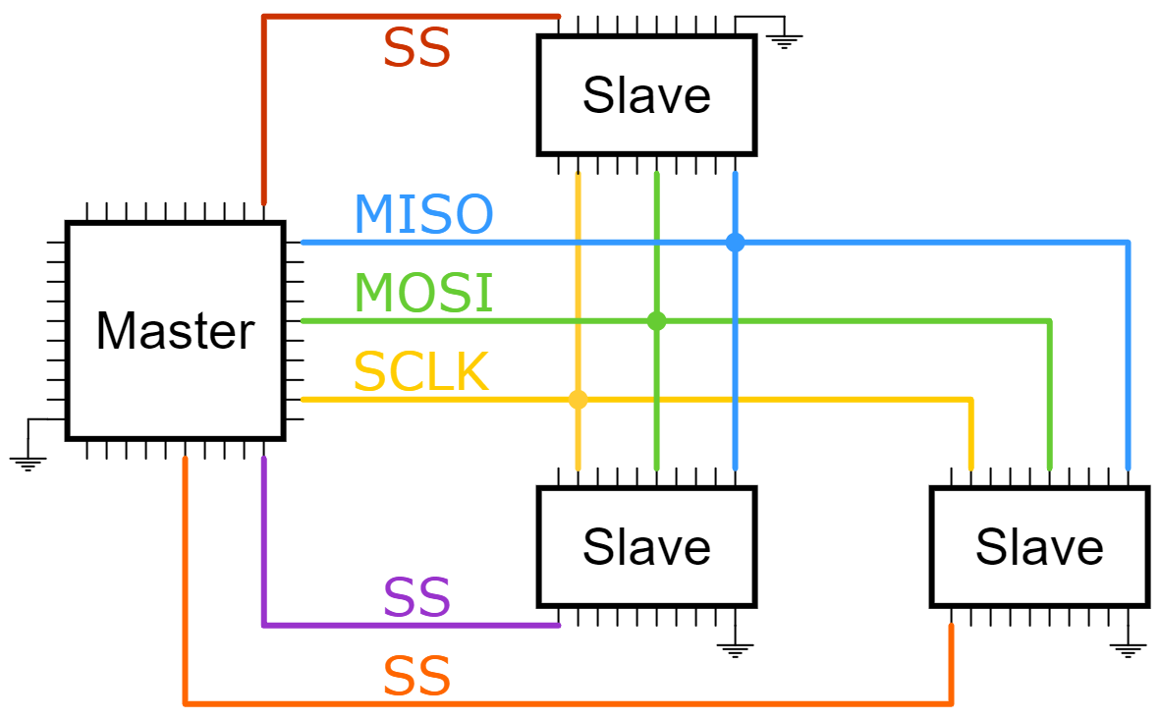
\includegraphics[width=0.9\textwidth]{images/spiWiring.png}}
    \caption[Zapojenie zbernice SPI]{Zapojenie zbernice SPI.}
    \label{obr:spiWiring}
\end{figure}

\section{Komunikácia s pamäťou AT93C66A}
Integrovaný obvod AT93C66A je jednoduchá pamäť typu EEPROM vyvinutá spoločnosťou Atmel. Veľkosť pamäte je 512 byte-ov, ktoré môžu byť organizované v 16-bitových slovách (words). Táto konfigurácia je nastaviteľná pomocou špeciálneho ORG pinu a je meniteľná za behu (atomicky vzhľadom na jednu inštrukciu) \cite{eepromDatasheet}.

\subsection{Inštrukčná sada}
AT93C66A je pamäť typu flash, preto rozlišuje dve rôzne operácie zápisu -- naprogramovanie (program) a zmazanie (erase). Naprogramovanie umožňuje nastavenie ktoréhokoľvek bitu vrámci adresovaného bloku (byte resp. slovo v závislosti od konfigurácie) na logickú hodnotu 0. Operácia zmazania umožňuje jednorázovo nastaviť celý adresovaný blok na logické hodnoty 1. 

Zápis do pamäte AT93C66A je preto možný realizovať pomocou dvoch inštrukcií. Inštrukcia ERASE umožňuje nastaviť všetky bity v jednom bloku pamäte (8 alebo 16 bitov v závislosti od konfigurácie pamäte) na logické hodnoty 1. Inštrukcia WRITE umožňuje zapísať na daný blok ľubovoľnú hodnotu. V prípade, že pri zápise nie je potrebné vykonať zmenu bitu s hodnotou 0 na hodnotu 1, inštrukcia WRITE je interne realizovaná priamo operáciou naprogramovania. V opačnom prípade musí operácií naprogramovania predchádzať operácia zmazania, ktorú v tomto prípade pamäť implicitne vykoná, pred samotným zápisom (efektívne vykoná inštrukciu ERASE, pred samotnou inštrukciou WRITE). V tomto prípade možno očakávať, že operácia zápisu bude trvať dlhšie, podrobnosti však výrobca v technickom liste neuvádza. V obidvoch prípadoch výrobca garantuje, že inštrukcia WRITE trvá najviac 10\,ms \cite{eepromDatasheet}. Okrem spomenutých inštrukcií, obsahuje inštrukčná sada AT93C66A aj ďalšie inštrukcie, popísané v tabuľke \ref{tab:eepromIS}.

\begin{table}[!h]
    \caption[Inštrukčná sada pamäte AT93C66A]{Inštrukčná sada pamäte AT93C66A \cite{eepromDatasheet}. Veľkosť bloku závisí na konfigurácií organizácie -- 8/16 bitov.}
    \label{tab:eepromIS}
    \begin{center}
    \begin{tabular}{V{4}c|c|c|cV{4}}
        \hlineB{4}
        Inštrukcia & Kód & Operandy & Popis \\
        \hlineB{4}
        READ & 10 & adresa & Prečíta blok dát uložený na danej adrese. \\
        \hline
        WRITE & 01 & adresa a blok dát & Zapíše blok na danú adresu. \\
        \hline
        ERASE & 11 & adresa & Na danej adrese nastaví všetky bity na 1. \\
        \hline
        WRAL & 0001 & blok dát & Zapíše hodnotu bloku na každú adresu. \\
        \hline
        ERAL & 0010 & -- & Vymaže pamäť. (Nastaví všetky bity na 1). \\
        \hline
        EWEN & 0011 & -- & Povolí všetky zápisové operácie.\\
        \hline
        EWDS & 0000 & -- & Zakáže všetky zápisové operácie.\\
        \hline
        \hlineB{4}
    \end{tabular}
    \end{center}
\end{table}

\subsection{Zbernica a komunikačný protokol}
Rozhranie pre komunikáciu s pamäťou využíva SPI zbernicu, pričom vodiče sú v technickom liste (angl. datasheet) označené CS (Chip Select), DI (zodpovedá MOSI), DO (zodpovedá MISO) a SK (SCLK) \cite{eepromDatasheet}. V pasívnom stave je na linke CS logická 0, čo nie je v súlade s väčšinou implementácií SPI zbernice. (Pripomíname, že SPI zbernica je defakto štandard.) Frekvencia hodinového signálu na SK linke musí byť z rozsahu 0,25--2\,MHz \cite{eepromDatasheet}. Schéma vývodov (angl. pinout) je na obrázku \ref{obr:eepromPinout}.

\begin{figure}[h!]
    \centerline{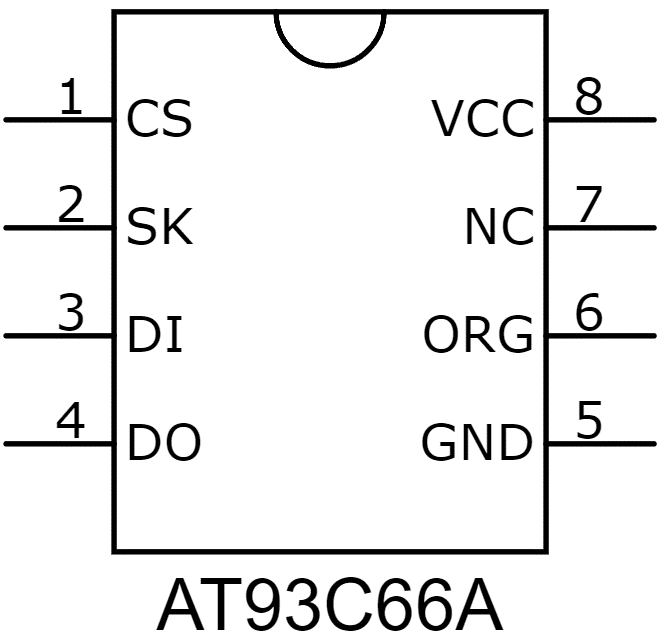
\includegraphics[width=0.25\textwidth]{images/at93c66aPinout.png}}
    \caption[Schéma vývodov pamäte AT93C66A]{Schéma vývodov pamäte AT93C66A. Pin NC (No Connect) je nevyužitý \cite{eepromDatasheet}.}
    \label{obr:eepromPinout}
\end{figure}

Komunikačný protokol pamäte AT93C66A je veľmi jednoduchý. Komunikácia je iniciovaná nábehovou hranou na CS vodiči a následným poslaním START bitu na DI. Na DI linke nasleduje kód inštrukcie a prípadné operandy (adresa a pri zápise aj obsah) \cite{eepromDatasheet}. V tabuľke \ref{tab:eepromIS} si možno všimnúť, že inštrukcie využívajú prefixový kód, čo umožňuje jednoznačne určiť inštrukciu a následne jej operandy, ktorých dĺžka už je jednoznačne určená z kontextu inštrukcie. Vstup (na DI linke) je vzorkovaný v vždy s nábehovou hranou na SK linke s hodinovým signálom. Počas posielania inštrukcie musí byť na CS vodiči napätie na úrovni logickej 1.

Nasledujúca časť komunikácie závisí od zadanej inštrukcie. V prípade inštrukcie READ, začne pamäť posielať prečítané bity po DO linke hneď po zadaní inštrukcie (s nasledujúcou nábehovou hranou na SK linke). Výstup je synchronizovaný vždy s nábehovou hranou operácie čítania a je predchádza mu jeden tzv. \uv{dummy} bit s hodnotou 0, ktorý sa na DO linke objaví súčasne s posledným bitom inštrukcie (v tomto prípade posledný bit zadanej adresy) na DI linke. Počas toho ako pamäť posiela výstup musí byť hodnota na CS vodiči rovná logickej 1. Po skončení operácie čítania musí napätie na CS vodiči klesnúť na úroveň logickej 0 a zotrvať minimálne po dobu 250\,ns, pred začatím ďalšej komunikácie. Komunikačný protokol v prípade inštrukcie READ je znázornený na obrázku \ref{obr:eepromREAD}. V prípade inštrukcie READ je možné ponechať napätie na CS linke na úrovni logickej 1 aj po prijatí posledného bitu prečítaných dát. V tom prípade s následujúcim taktom na SK linke začne pamäť automaticky posielať po DO linke obsah na nasledujúcej adrese. Takýmto spôsobom je možné sekvenčne prečítať pamäť až po poslednú adresu.

\begin{figure}
    \centerline{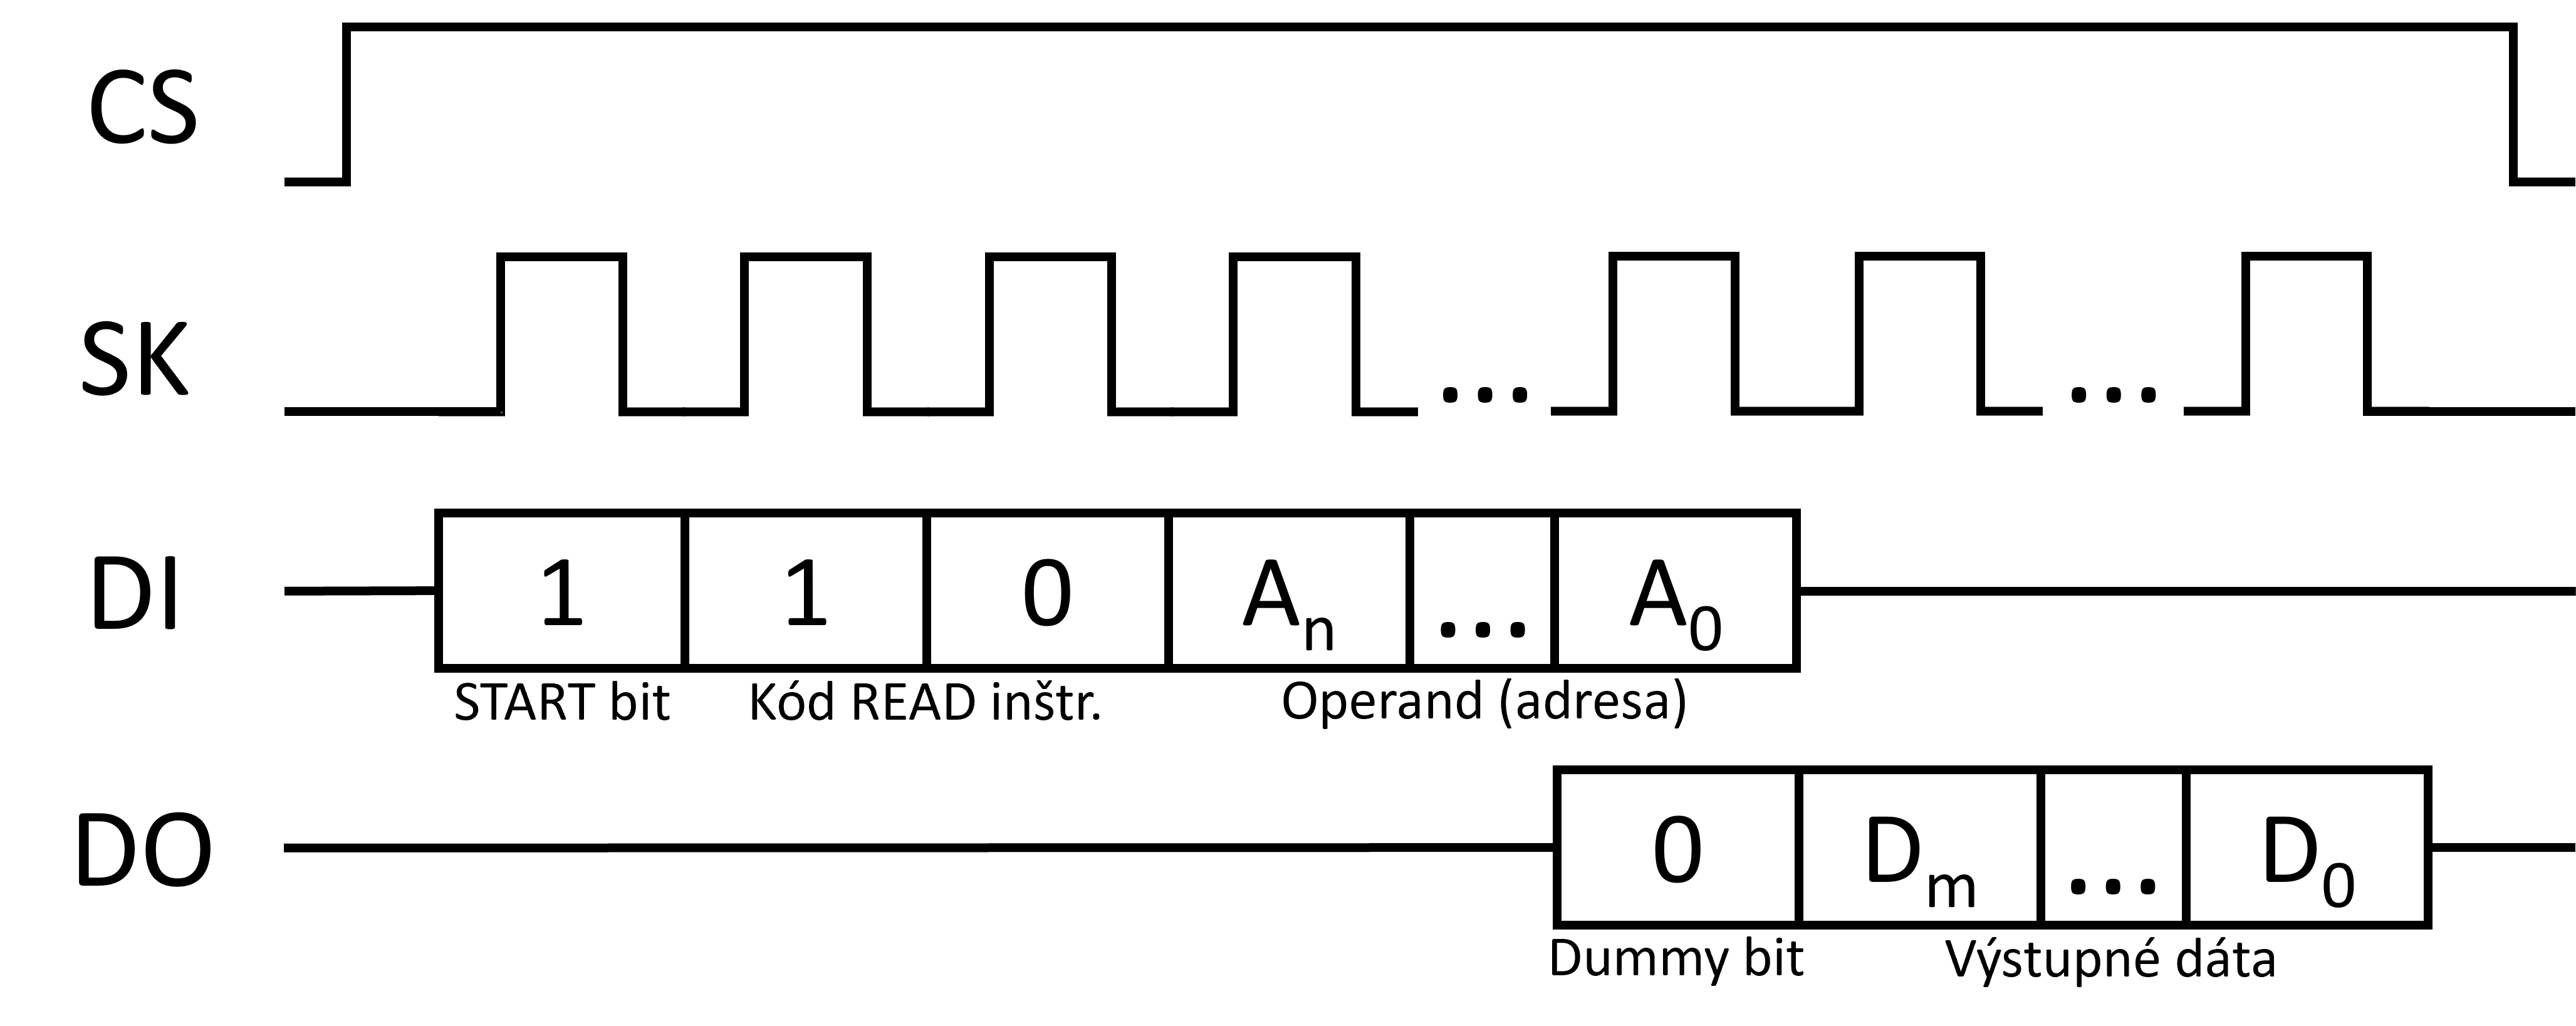
\includegraphics[width=1\textwidth]{images/eepromREAD.png}}
    \caption[Protokol pre čítanie pamäte AT93C66A]{Protokol pre čítanie pamäte AT93C66A. Na obrázku je znázornená komunikácia na jednotlivých linkách v čase. Adresa aj dáta sú posielané od najvyššieho bitu k najnižšiemu.}
    \label{obr:eepromREAD}
\end{figure}

V prípade inštrukcií zápisu WRITE, ERASE, WRAl a ERAL si pamäť vyhradzuje čas potrebný pre vykonanie inštrukcie (0,1 -- 10\,ms \cite{eepromDatasheet}). Tieto inštrukcie neprodukujú žiaden výstup, preto je komunikáciu možné ukončiť ihneď po zadaní inštrukcie nastavením logickej 0 na CS vodiči (minimálne po dobu 250\,ns ako v prípade READ inštrukcie). Pri nasledujúcej nábehovej hrane na CS vodiči (teda pokus o iniciovanie ďalšej komunikácie) začne pamäť na DO linke posielať tzv. READY/BUSY bit (synchronizovaný vždy na nábehovú hranu SK linky). Pokiaľ je pamäť pripravená na vykonanie ďalšej inštrukcie (READY), pošle bit s hodnotou 1, pokiaľ je zaneprázdnená (BUSY) vykonávaním predošlej inštrukcie, pošle bit s hodnotou 0. Takýmto spôsobom je možné opakovane testovať stav pamäte vždy s nábehovou hranou na SK linke. Počas tejto doby musí byť napätie na SC vodiči na úrovni logickej 1. Pokiaľ nábehová hrana na CS vodiči príde až po uplynutí vyhradeného času pre vykonanie inštrukcie, ktorý trvá minimálne 0,1\,ms, READY/BUSY komunikáciu už nie je možné iniciovať a pamäť očakáva ďalšiu inštrukciu. Opisaná komunikácia v prípade inštrukcií zápisu je znázornená na obrázku \ref{obr:eepromWRITE}.

\begin{figure}[h!]
    \centerline{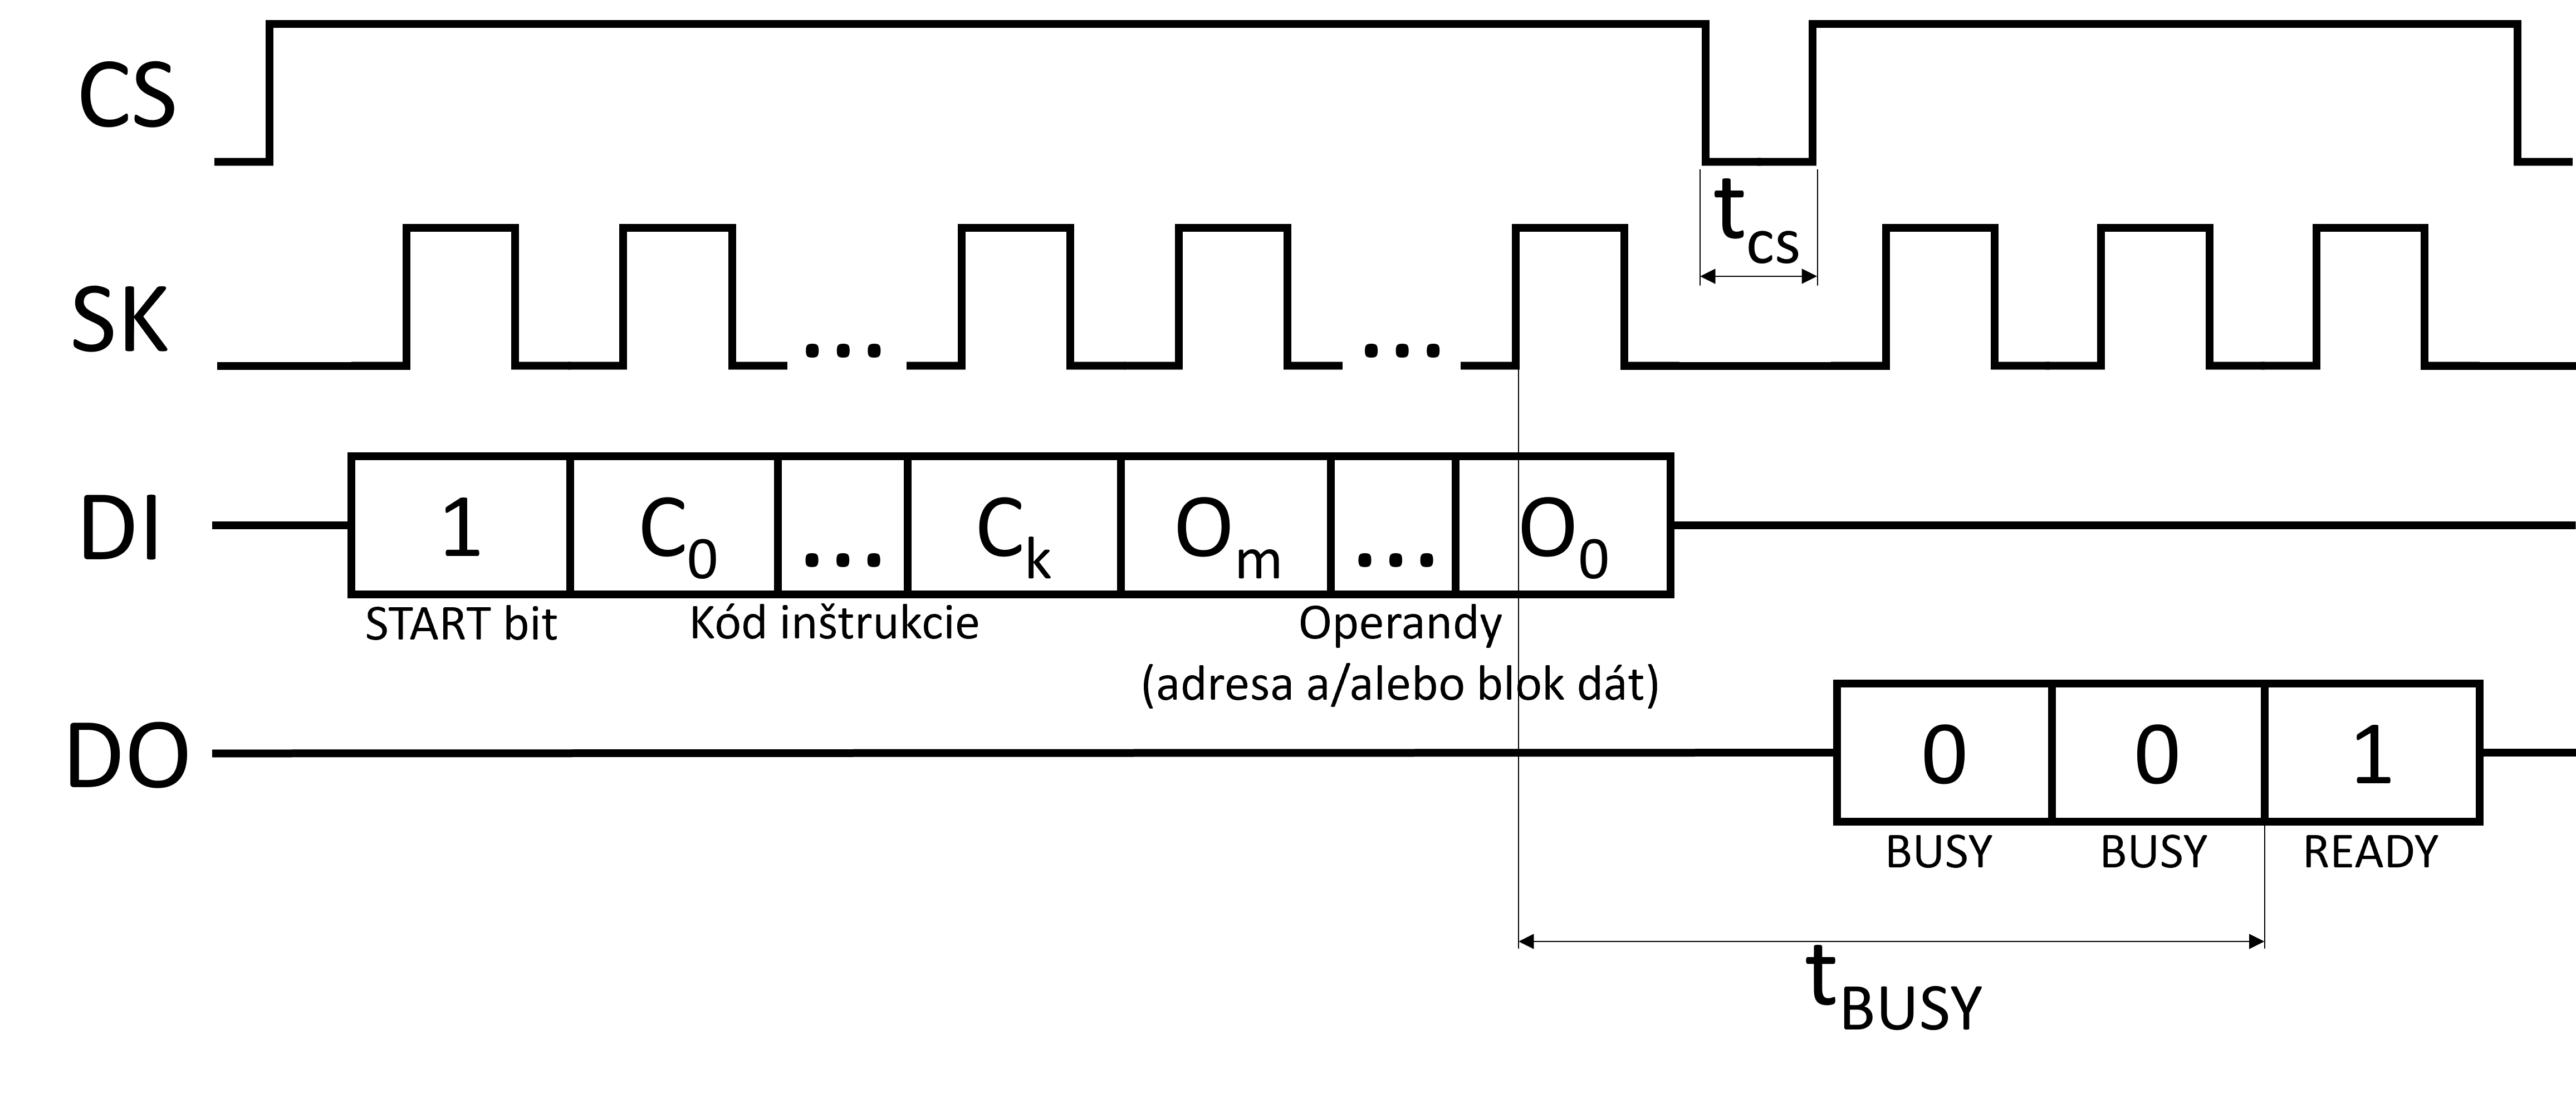
\includegraphics[width=1\textwidth]{images/eepromWRITE.png}}
    \caption[Protokol pre zápis do pamäte AT93C66A]{Protokol pre zápis do pamäte AT93C66A. Na obrázku je znázornená komunikácia na jednotlivých linkách v čase. Operandy sú posielané od najvyššieho bitu k najnižšiemu. Interval t\textsubscript{CS} je minimálne 250\,ns a t\textsubscript{BUSY} je z rozsahu 0,1 -- 10\,ms.}
    \label{obr:eepromWRITE}
\end{figure}

Inštrukcie EWEN a EWDS neprodukujú žiaden výstup a nevyhradzujú žiaden čas potrebný pre ich vykonanie. Po zadaní týchto inštrukcií preto možno komunikáciu ihneď ukončiť a následne iniciovať ďalšiu (opäť nastavením logickej 0 po dobu minimálne 250\,ns na CS vodiči).